\appendix
\chapter{Example Tree of Some $\mathcal{Q}$}
\label{app:tree}
\centering
\begin{minipage}{0.49\linewidth}
\centering
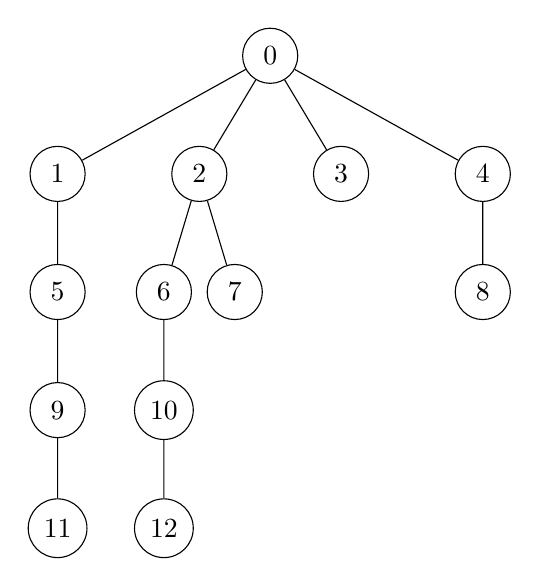
\begin{tikzpicture}[level/.style={sibling distance=18mm/#1}]
\tikzset{every node/.style={shape=circle,draw,minimum size=7mm}}
%\tikzset{every node/.style={shape=circle,
%                            font=\bfseries \Large,
%                            minimum size=3cm,
%                            scale=0.4
%                           }}
\node (root) {$0$}
    child {node (n1) {$1$}
        child {node (n5) {$5$}
            child {node (n9) {$9$}
                child {node (11) {$11$}
                }
            }
        }
    }
    child {node (n2) {$2$}
        child {node (n6) {$6$}
            child {node (n10) {$10$}
                child {node (n12) {$12$}
                }
            }
        }
        child {node (n7) {$7$}
        }
    }
    child {node (n3) {$3$}
    }
    child {node (n4) {$4$}
        child {node (n8) {$8$}
        }
    }
    ;
\end{tikzpicture}
\end{minipage}
\begin{minipage}{0.5\linewidth}
\centering
\begin{tabular}{rll}
         $k$ & $\mathcal{M}_k$            & $\mathcal{Z}_k$ \\ \hline
    0        & $\left\{{}\right\}$        & $\left\{{1,3}\right\}$ \\
    1        & $\left\{{2}\right\}$       & $\left\{{2,3,5}\right\}$ \\
    2        & $\left\{{4}\right\}$       & $\left\{{4,1,5}\right\}$ \\
    3        & $\left\{{5}\right\}$       & $\left\{{5,1,3}\right\}$ \\
    4        & $\left\{{2,4}\right\}$     & $\left\{{2,4,3,5}\right\}$ \\
    5        & $\left\{{2,1}\right\}$     & $\left\{{2,1,4,5}\right\}$ \\
    6        & $\left\{{4,3}\right\}$     & $\left\{{4,3,1}\right\}$ \\
    7        & $\left\{{4,2,3}\right\}$   & $\left\{{4,2,3,5}\right\}$ \\
    8        & $\left\{{2,4,1}\right\}$   & $\left\{{2,4,1,3}\right\}$ \\
    9        & $\left\{{2,1,3}\right\}$   & $\left\{{2,1,3,4}\right\}$ \\
    10       & $\left\{{4,3,5}\right\}$   & $\left\{{4,3,5,2}\right\}$ \\
    11       & $\left\{{2,1,3,5}\right\}$ & $\left\{{2,1,3,5}\right\}$ \\
    12       & $\left\{{4,3,5,1}\right\}$ & $\left\{{4,3,5,1,2}\right\}$
\end{tabular}
\end{minipage}


\chapter{Slp Header Files}

\section*{\texttt{Algorithm.hpp}}
\begin{verbatim}
/**
 * Perform a line search by finding the minimum objective value
 * of the given QP problem of all the points between the two
 * given points.
 *
 * @param  p1
 *         Start point.
 * @param  p2
 *         End point.
 * @param  model
 *         ClpModel of the QP problem.
 * @return the step length alpha.
 */
double lineSearch(double* p1, double* p2, const ClpModel model);
\end{verbatim}

\begin{verbatim}
/**
 * Solve a QP problem using Slp.
 *
 * @param  quad
 *         ClpModel containing the QP problem.
 * @param  x
 *         Array containing the initial guess vector. This array
 *         will be overwritten with a final solution.
 * @param  maxIters
 *         Number of iterations to perform if the stopping
 *         criteria is not met.
 * @param  tol
 *         Epsilon for the stopping criteria.
 * @return the objective value of the solved QP problem..
 */
double solve(ClpModel quad, double* x, int maxIters, double tol);
\end{verbatim}

\newpage

\begin{verbatim}
/**
 * Perform a Taylor-series expansion of the objective function of
 * the given QP problem at the given point.
 *
 * @param destCoeffs
 *        Pointer to coefficient destination.
 * @param point
 *        Point to perform the expansion at.
 * @param model
 *        ClpModel that has the objective function.
 */
void taylor(double* destCoeffs, double* point, ClpModel model);
\end{verbatim}

\begin{verbatim}
/**
 * Evaluate the objective function of the given model at
 * the given point.
 *
 * @param point
 *        Point to evaluate the objective function at.
 * @param model
 *        ClpModel that has the objective function to evaluate.
 */
doubld value(double* point, ClpModel model);
\end{verbatim}
